\chapter{Experiments}\label{chap:experiments}

Experiments were run on a Server with the following specs (Specifics
here\footnote{\url{https://ark.intel.com/content/www/us/en/ark/products/92981/intel-xeon-processor-e5-2630-v4-25m-cache-2-20-ghz.html},
accessed 2019-06-26}):

\begin{table}[ht]
    \ra{1.3}
\begin{tabular}{@{}lr@{}}
    Processor & Intel® Xeon® Processor E5 v4 Family \\
    Number & E5-2630V4 \\ \midrule
    \textbf{Performance} & \\ \midrule
    Number of Cores & 10 \\
    Number of Threads & 20 \\
    Base frequency & 2.2 GHz \\
    Max Turbo frequency & 3.1 GHz \\
    Working Memory (RAM) & 120 GByte \\
\end{tabular}
\end{table}


% Experiments
\todo{The time-resource-measures done}


\begin{figure}[t]
\begin{centering}
    \subfloat[Pairplot over some variables]
    {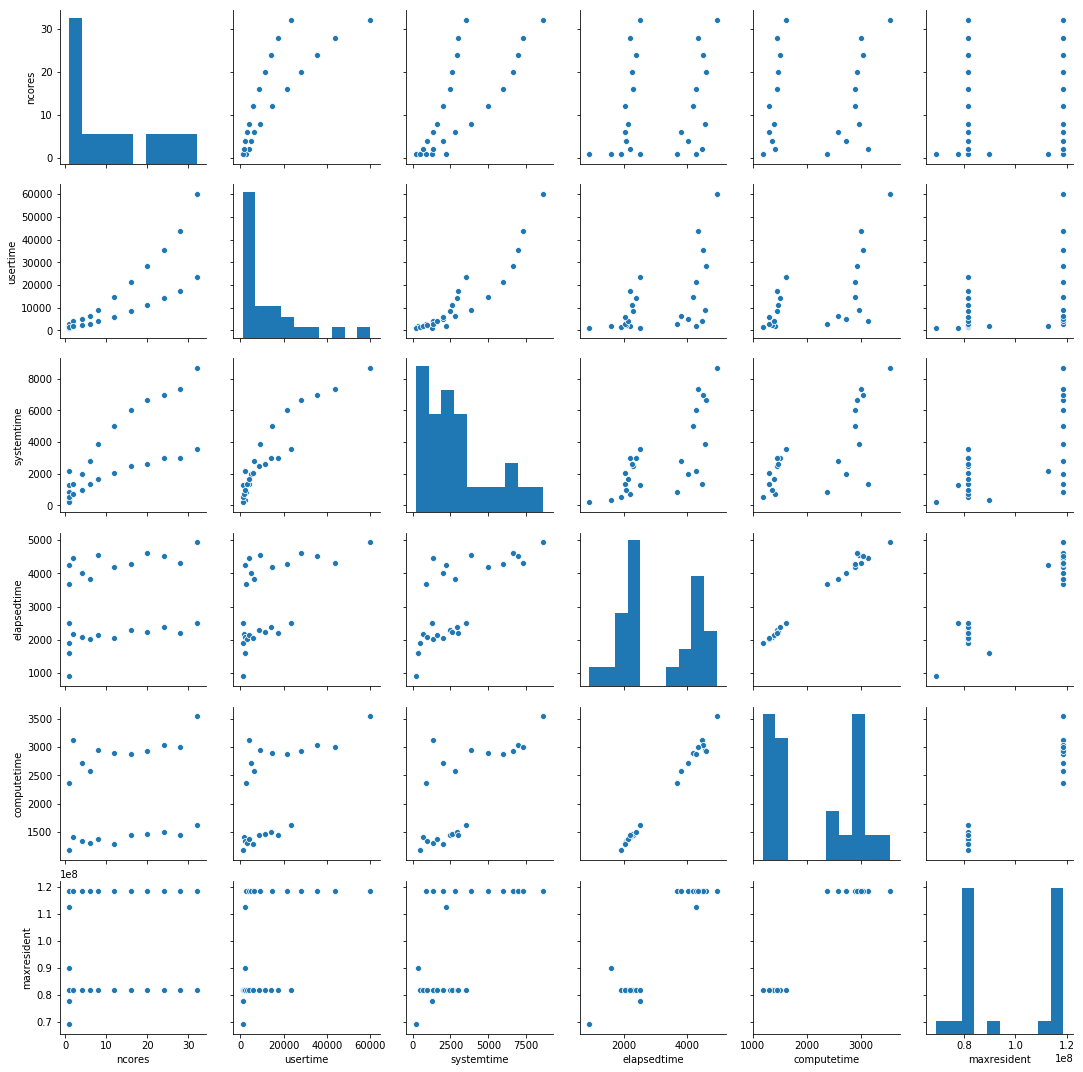
\includegraphics[scale=0.5]{figures/experiments/pairplot.png}}
    \caption[Pairplot]{\textbf{Pairplot over some of the variables ...} moar info here}
    \label{fig:pairplot}
\end{centering}
\end{figure}


\draft{Something is off with my numbers, they show something entirely different from earlier. I'll check that again.}

See \figref{fig:pairplot} (more of that will follow).

\todo{add where the matrices / data is from}

\todo{graphics: runtime vs cores (RUST), RAM vs variants, runtime vs variants}

\todo{add plot of matrix uncorrected vs corrected ice vs corrected KR vs corrected ice\_rust}

% using hicPlotMatrix -m <matrixname> --region 1:18000000-22000000 --log1p -o <outfile>.png

% \subsection{Testing}\label{sec:testing}

% \todo{Rewrite to passive voice}

% I ran a total of 416 different configurations to test for a total of 3
% different parameters. The first two are the same for all, the third applies
% only to this implementation. I tested the original Python-implementation as
% well as the new KR in C++.

% \begin{itemize}
%     \item Size of Matrix (four different ones)
%     \item Number of chromosomes (8 different sizes)
%     \item Number of threads (11 different numbers)
% \end{itemize}

% \todo{add: data is primary data, from: GM12878 something rao2014}

% \newpage
% The sizes of the matrices for reference (biggest to smallest):

% \begin{verbatim}
% # Matrix information file. Created with HiCExplorer's hicInfo version 3.0
% File:   matrix.h5
% Size:   309,581
% Bin_length:     10000
% Sum of matrix:  2416588411.2530212
% Chromosomes:    1, 2, 3, 4, 5, 6, 7, 8, 9, 10, 11, 12, 13,
%                 14, 15, 16, 17, 18, 19, 20, 21, 22, X, Y, MT
% Non-zero elements:      2,111,867,476
% Minimum (non zero):     0.008667398294551536
% Maximum:        139544.65657933566
% NaN bins:       25948

% # Matrix information file. Created with HiCExplorer's hicInfo version 3.0
% File:   25kb_raw.h5
% Size:   123,841
% Bin_length:     25000
% Sum of matrix:  2378265786.0
% Chromosomes:    1, 2, 3, 4, 5, 6, 7, 8, 9, 10, 11, 12, 13,
%                 14, 15, 16, 17, 18, 19, 20, 21, 22, X, Y, MT
% Non-zero elements:      1,530,533,003
% Minimum (non zero):     1
% Maximum:        320932
% NaN bins:       9290
% \end{verbatim}
% \newpage
% \begin{verbatim}
% # Matrix information file. Created with HiCExplorer's hicInfo version 3.0
% File:   50kb_raw.h5
% Size:   61,928
% Bin_length:     50000
% Sum of matrix:  2333794628.0
% Chromosomes:    1, 2, 3, 4, 5, 6, 7, 8, 9, 10, 11, 12, 13,
%                 14, 15, 16, 17, 18, 19, 20, 21, 22, X, Y, MT
% Non-zero elements:      1,053,216,825
% Minimum (non zero):     1
% Maximum:        320932
% NaN bins:       4514

% # Matrix information file. Created with HiCExplorer's hicInfo version 3.0
% File:   small_test_matrix.h5
% Size:   33,754
% Bin_length:     5000
% Sum of matrix:  35778.0
% Chromosomes:    chr2RHet, chr3RHet, chr2LHet, chr4, chrYHet, chr3L, chr2L,
%                 chrU, chrX, chrXHet, chr2R, chr3R, chrUextra, chrM, chr3LHet
% Non-zero elements:      69,213
% Minimum (non zero):     1
% Maximum:        8
% NaN bins:       0
% \end{verbatim}

% \todo{remove this verbatim part and make table instead}

% \extend{building matrix-test-suite and getting results}



\todo{mention that data is from rao20143d}

